\section{Appendix}
\frame{Appendix}


\begin{frame}{Bayesian Learning}
    \frametitle{Posterior Distribution: Markov Chain Monte Carlo}
    \begin{columns}
      \begin{column}{0.45\linewidth}
        \begin{itemize}
          \item \textcolor{green}{Markov Chain Monte Carlo (MCMC) methods}: estimate the
          exact posterior distribution by drawing samples generated from a Markov
          chain.
          \item The samples are accepted or rejected based on a criterion. 
          % \item This criterion is chosen to ensure that the stationary
          % distribution of the Markov chain is the posterior distribution.
        \end{itemize}
      \end{column}
      \begin{column}{0.55\linewidth}
        \includegraphics[width=0.9\linewidth]{mcmc.png}
      \end{column}
    \end{columns}
    \footnotetext[1]{Jin, Seung-Seop \& Ju, Heekun \& Jung, Hyung-Jo. (2019). Adaptive Markov chain Monte Carlo algorithms for Bayesian inference: recent advances and comparative study. Structure and Infrastructure Engineering. 10.1080/15732479.2019.1628077.}
\end{frame}

% \begin{frame}{Bayesian Learning}
%     \frametitle{Posterior Distribution: Variational Inference}
%     \begin{itemize}
%       \item \textcolor{green}{Variational inference}: given the form of the
%       likelihood and the prior distributions, the posterior distribution $q(\theta;z)$
%       is chosen from the conjugate family.
%       \item The objective is to learn the distribution parameters $z$, such that
%       the \textit{evidence lower bound} (\textsc{Elbo}) given by
%       \begin{align*}
%           \mathcal{L}(\mathcal{D},z) = \mathbb{E}_{\theta \sim q} \left[\log( p(\mathcal{D} \mid \theta;z)p(\theta;z)) - \log(q(\theta;z)) \right]
%       \end{align*}
%       is maximized.
%       \item \textbf{Note}: Maximizing \textsc{Elbo} is similar to minimizing the Kullback-Leibler divergence, which is 
%       \begin{align*}
%         D_{KL} &= \mathbb{E}_{\theta \sim q}\left [ \log \frac{q(\theta)}{p(\theta \mid \mathcal{D})} \right] \\
%         &= \log(p({\mathcal{D})}) - \mathbb{E}_{\theta \sim q} \left[ \log \frac{ p(\mathcal{D} \mid \theta;z)p(\theta;z)}{q(\theta)}\right]
%       \end{align*}
%     \end{itemize}
% \end{frame}

\begin{frame}{\textsc{IdaPbc}} 
  \begin{itemize}
    \item The system's equations of motion can then be expressed as 
    %
    \begin{align}
        \begin{split}  
          \bmat{\dot{q} \\ \dot{p}} &= \bmat{0 & I_n \\ -I_n & 0}\bmat{\nabla_qH \\
          \nabla_pH} + \bmat{0 \\ G(q)}u,
          % y &= G^\top \dot{q},
        \end{split}
        \label{eq:hamiltonian_dynamics}
    \end{align}
    %
    where $G(q) \in \mathbb{R}^{n \times m}$ is the input matrix, $I_n$ is the
    $n \times n$ identity matrix, and $u \in \mathcal{U} \subset \mathbb{R}^m$ is
    the control input.
    \item In \textsc{IdaPbc}, the closed-loop dynamics is
    chosen as the port-controlled Hamiltonian (PCH) form:
    %
    \begin{equation}
      \bmat{\dot{q} \\ \dot{p}}
      =
    %   \bmat{J_d(q,p) - R_d(q,p)}
      \bmat{0 & M^{-1}M_d \\ -M_dM^{-1} & J_2(q,p) - GK_vG^\top}
      \bmat{\nabla_q H_d \\ \nabla_p H_d},
      \label{eq:pch}
    \end{equation}
    %
    where $J_2 = -J_2^\top$
  \end{itemize}
  
\end{frame}

\begin{frame}{Tracking Trajectory}
    \begin{itemize}
        \item Let $\gamma : t \rightarrow \phi(t;x_0, u^\theta)$ represent the flow of the dynamical system
        \item The objective is to track an expert trajectory $\gamma^\star$ provided by a path planner 
        \item The running cost that achieves this is given by 
        \begin{align*}
            J_{track}(\gamma_\bot) &= \sum_{x_\bot \in \gamma_\bot, \; x^\star_\bot \in \gamma^\star_\bot} |\left| x_\bot-x^\star_\bot | \right |^2  
        \end{align*}
        where $(\cdot)_\bot$ expresses the state in transverse coordinates along the desired orbit $\gamma^\star$
        \item The corresponding likelihood is 
        \begin{align*}
            p(\mathcal{D} \mid \theta) &= p(\gamma_\bot | \theta) = \prod_{x_\bot \in \gamma_\bot, \; x^\star_\bot \in \gamma^\star_\bot}\mathcal{N}(x^\star_\bot , \Sigma) \\
            &= \prod_{x_\bot \in \gamma_\bot, \; x^\star_\bot \in \gamma^\star_\bot} \frac{1}{\sqrt{|2\pi \Sigma|}} e^{-\frac{1}{2}(x_\bot - x^\star_\bot)^\top \Sigma^{-1} (x_\bot - x^\star_\bot)}
        \end{align*}
    \end{itemize}
\end{frame}


% \begin{frame}[fragile]
%     \frametitle{Neural passivity-based control (\textsc{NeuralPbc})}
%     \begin{columns}
%         \begin{column}[c]{0.62\linewidth}
%             \begin{exampleblock}{Main Learning Problem}
%             % \begin{small}
%                 \begin{equation*}
%                     \begin{aligned}
%                         \underset{\theta}{\textrm{minimize}} 
%                         & & &\int_{0}^{T} \ell \left(\phi,u^{\theta}(\phi) \right) \, \dd t , \\%
%                         \textrm{subject to}
%                         & & \dot{x} &= \bmat{\phantom{-}\nabla_p H \\ -\nabla_q H} + \bmat{0 \\ G(q)}u^{\theta}, \\%
%                         & & u^{\theta} &= -G^{\dagger} \nabla_q H_d^{\theta} - K_v^{\theta} G^\top \nabla_p H_d^{\theta},%
%                         % & \quad x(0) &= x_0 \in \mathcal{X}, \\%
%                     \end{aligned}
%                 \end{equation*}
%                 $H_d^\theta$ is parametrized by a \textit{stochastic} neural network
%             % \end{small}
%             \end{exampleblock}
%         \end{column}
%         \begin{column}[c]{0.36\linewidth}
            
%         \end{column}
%     \end{columns}
% \end{frame}

% \begin{frame}
%     \begin{columns}
%         \begin{column}{0.62\linewidth}
%             \begin{figure}
%                 \centering
%                 \includegraphics[width=0.8\linewidth]{figures/bandplot2.eps}
%             \end{figure}
%         \end{column}
%         \begin{column}{0.36\linewidth}
%         \end{column}
%     \end{columns}
% \end{frame}

% \begin{frame}{ \textsc{NeuralPbc}}
%     \begin{columns}
%         \begin{column}{0.48\linewidth}
%             \begin{table}[tb]
%                 \centering
%                 \footnotesize
%                 \caption{System parameters used in real-world experiments. The errors in the
%                 last column are $\|p_s - p^{\textrm{nom}}_{s}\| / \|p^{\textrm{nom}}_{s}\|$}.
%                 % \rowcolors{2}{}{Wheat1}
%                 \begin{tabular}{lcccc}
%                   \toprule
%                   Parameter set $p_s$ & $I_1$ & $I_2$ & $mgl$ & Error \\
%                   \midrule
%                   Nominal & 0.0455 & 0.00425 & 1.795 & 0 \\
%                   A & 0.0417 & 0.00330 & 1.577 & $0.122$ \\
%                   B & 0.0378 & 0.00235 & 1.358 & $0.243$ \\
%                   C & 0.0340 & 0.00141 & 1.140 & $0.365$ \\
%                   \bottomrule
%                 \end{tabular}
%                 \label{tab:modified_params}
%               \end{table}
%         \end{column}
%         \begin{column}{0.46\linewidth}
%             \begin{figure}
%                 \centering
%                 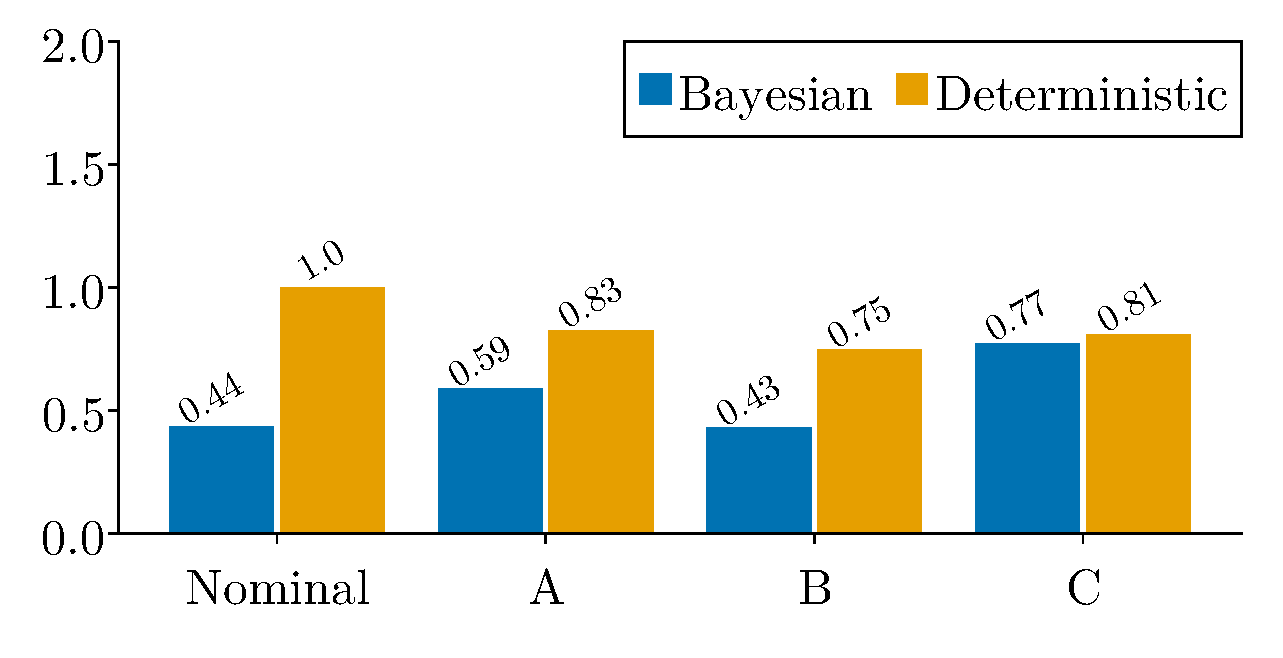
\includegraphics[width=0.9\linewidth]{figures/pbc_bar.eps}
%             \end{figure}
%         \end{column}
%     \end{columns}
% \end{frame}


% \begin{frame}{Running cost $J$}
%   \begin{itemize}
%     \item The performance objective $J$ can be one or combination of the following cost functions.
%   \end{itemize}
%   \begin{enumerate}
%     \item Loss to desired trajectory ($J_{track}$)
%     \item Terminal loss ($J_T$)
%     \item Set distance loss ($J_{set}$)
% \end{enumerate}
% \end{frame}

% \begin{frame}{Loss to desired trajectory ($J_{track}$)}
%     \begin{columns}[c]
%       \begin{column}{0.46\linewidth}
%         \begin{itemize}
%           \item Loss to desired trajectory ($J_{track}$) : tracks expert trajectory $\gamma^*$
%           \begin{align*}
%             J_{track}(\gamma_\bot) &= \sum_{x_\bot \in \gamma_\bot, \; x^\star_\bot \in \gamma^\star_\bot} |\left| x_\bot-x^\star_\bot | \right |^2 \\
%             p(\mathcal{D}, \theta) &= p(\gamma_\bot | \theta) = \prod_{x_\bot \in \gamma_\bot, \; x^\star_\bot \in \gamma^\star_\bot}\mathcal{N}(x^\star_\bot , \Sigma).
%           \end{align*}
%         \end{itemize}
%       \end{column}
%       \begin{column}{0.48\linewidth}
%       \end{column}
%     \end{columns}
% \end{frame}


% \begin{frame}{Sampling initial states}

% \end{frame}

